\documentclass[a4paper,12pt]{article}

% Pacchetti necessari
\usepackage[utf8]{inputenc}
\usepackage{graphicx}
\usepackage{amsmath}
\usepackage{hyperref}
\usepackage{listings}
\usepackage{float}
\usepackage{caption}
\usepackage{subcaption}
\usepackage{booktabs}
\usepackage{xcolor}
\usepackage{geometry}

% Definizione dei colori per il codice
\definecolor{codebg}{rgb}{0.95, 0.95, 0.95}
\definecolor{codecmnt}{rgb}{0.25, 0.5, 0.35} % Commenti più scuri
\definecolor{codekw}{rgb}{0.2, 0.4, 0.8} % Parole chiave con un blu meno brillante
\definecolor{codeid}{rgb}{0.6, 0.4, 0.8} % Identificatori meno sgargianti
\definecolor{codegray}{rgb}{0.4, 0.4, 0.4} % Numeri di riga meno intensi

% Stile personalizzato per il codice
\lstdefinestyle{mystyle}{
    backgroundcolor=\color{codebg},   
    commentstyle=\color{codecmnt},
    keywordstyle=\color{codekw},
    numberstyle=\tiny\color{codegray},
    stringstyle=\color{codeid},
    basicstyle=\ttfamily\footnotesize,
    breaklines=true,
    captionpos=b,                    
    keepspaces=true,                 
    numbers=left,                    
    numbersep=5pt,                  
    showspaces=false,                
    showstringspaces=false,
    tabsize=2
}

\lstset{style=mystyle}

% Impostazione dei link senza bordo
\hypersetup{
    colorlinks=true,
    linkcolor=black,
    filecolor=black,      
    urlcolor=blue,
    pdfborder={0 0 0}, % Elimina il contorno dei link
}

% Impostazione delle dimensioni della pagina
\geometry{
    a4paper, % Formato della pagina
    left=2.5cm, % Margine sinistro
    right=2.5cm, % Margine destro
    top=3cm, % Margine superiore
    bottom=3cm, % Margine inferiore
}

% Titolo del documento
\title{
    \vspace{-2cm} % Spazio per allineare correttamente l'intestazione
    \textbf{\Large Università degli Studi di Palermo} \\
    \vspace{0.3cm}
    \textbf{\Large Corso di Laurea in Informatica} \\
    \vspace{1cm}
    \textbf{\Large Esame di ``Laboratorio di Algoritmi''} \\
    \vspace{0.5cm}
    \textbf{\Large Relazione della prova pratica} \\
    \vspace{2cm}
    \textbf{Habasescu Alin Marian} \\
    \vspace{0.5cm}
    \textbf{\Large Soluzione prova pratica} \\
    \vspace{1cm}
}

\date{\normalsize Data di consegna: \today} % Data del documento

\begin{document}

\maketitle % Genera il titolo

\tableofcontents % Genera l'indice
\clearpage

\section{Soluzione proposta}
Il progetto richiede di minimizzare la perdita d'acqua nel trasporto tra acquedotti, 
modellando la rete idrica come un grafo pesato dove i nodi rappresentano gli acquedotti 
e i lati bidirezionali rappresentano le tubazioni con un determinato livello di perdita 
d'acqua espressa in millilitri al secondo. \\

Il problema principale sta nel voler calcolare i millilitri al secondo che vengono persi 
lungo una sequenza di tubi, da un certo acquedoto S ad un
altro acquedoto T, individuando la minor perdita possibile.\\

Per risolvere il problema, ho scelto di applicare l'algoritmo di Dijkstra, 
che è particolarmente adatto per trovare il percorso minimo in termini di peso,
da un vertice S detto ``sorgente'' ad un vertice T detto ``destinazione'', 
purché i pesi degli archi siano non negativi.\\

\subsection{Algoritmi e codici utilizzati}
Durante lo svolgimento del corso, mi è stato molto utile creare una repository GitHub
con diverse implementazioni di algoritmi e strutture dati. 
Per il completamento del progetto ho utilizzato alcuni algoritmi e strutture dati
da me stesso implementate, tra cui l'algoritmo di Dijkstra, la classe WeightedGraph,
la classe Heap.

Il codice sorgente completo può essere consultato al seguente link:

\begin{quote}
    \url{https://github.com/H-Alin02/DSA-in-cpp}
\end{quote}

All'interno del progetto, ho riutilizzato alcune classi precedentemente sviluppate 
per la gestione di grafi pesati e l'implementazione di algoritmi sui grafi. 
In particolare, ho utilizzato:

\begin{itemize}
    \item La classe \texttt{WeightedGraph} gestisce la struttura dati del 
    \textbf{grafo pesato}, che viene implementata tramite lista di adiacenza o 
    matrice di adiacenza. 

    \item L'algoritmo di \textbf{Dijkstra} per il calcolo del percorso minimo tra nodi 
    in un grafo pesato, che è stato implementato nella classe \texttt{GraphAlgorithms}.
\end{itemize}

\subsection{Algoritmo di Dijkstra}

L'algoritmo di Dijkstra per il calcolo del percorso minimo è stato implementato nella 
classe \texttt{GraphAlgorithms}. 
Di seguito è riportata una versione dell'algoritmo: 

\clearpage

\begin{lstlisting}[language=c++, label=Dijkstra]
    // Dijkstra implementation to find the shortest path from start to destination
    static int dijkstra(int start, int end, const GraphType& graph) {
        int nodes = graph.getVertices();

        if (start < 0 || start >= nodes || end < 0 || end >= nodes) {
            throw out_of_range("Invalid start or end node");
        }

        // Priority queue to select the node with the smallest distance
        Heap<pair<T, double>> pq(
            [](const pair<T, double>& a, const pair<T, double>& b) {
            return a.second < b.second;
        }, true);

        // Initialize distances to infinity
        vector<double> dist(nodes, numeric_limits<double>::infinity());
        dist[start] = 0;
        pq.push({start, 0});

        while (!pq.empty()) {
            int u = pq.top().first; 
            int u_dist = pq.top().second;
            pq.pop();

            if (u == end)
                return u_dist;

            for (const auto &neighbor : graph.getEdges(u)) {
                int v = neighbor.first.second;
                double weight = neighbor.second;

                if (dist[v] > u_dist + weight) {
                    dist[v] = u_dist + weight;
                    pq.push({v, dist[v]});
                }
            }
        }

        return -1;
    }


\end{lstlisting}

L'algoritmo utilizza una \textbf{coda di priorità} (Min-Heap) per estrarre il nodo con 
la distanza minore e aggiornare le distanze per i nodi adiacenti. Il codice gestisce sia grafi 
con lista di adiacenza che grafi pesati.\\

Nel contesto del progetto attuale, queste classi sono state riutilizzate per 
implementare una serie di funzionalità, tra cui il calcolo dei percorsi minimi tra 
i nodi e la visualizzazione di grafi pesati. Il riuso del codice ha consentito una 
notevole riduzione della complessità, poiché le classi e gli algoritmi erano già 
testati e ottimizzati.\\

Le implementazioni sono state facilmente adattate alle specifiche del progetto, 
permettendo l'integrazione efficiente di funzionalità come la gestione di grafi con 
pesi variabili e l'esecuzione di algoritmi di ricerca del percorso minimo.


\section{Correttezza dell'algoritmo}

Analiziamo ora la correttezza dell' implementazione dell'algoritmo di Dijkstra 
confrontandolo con il suo Pseudocodice originale: 

\begin{figure}[h!]
    \centering
    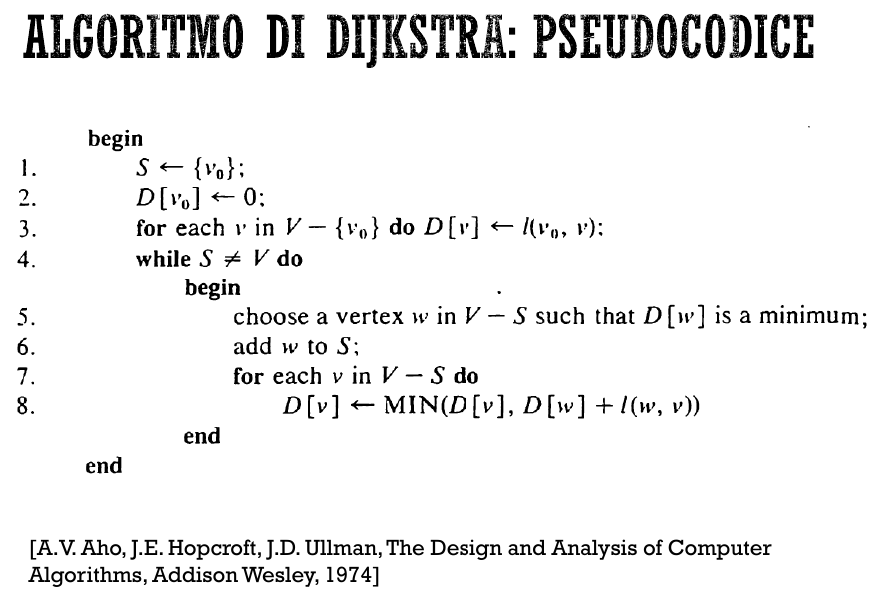
\includegraphics[width=0.7\textwidth]{Images/DijkstraPseudoCode.png}
    \caption{Pseudocodice dell'algoritmo di Dijkstra.}\label{fig:Pseudocodice Dijkstra}
\end{figure}


\begin{enumerate}
    \item \textbf{Inizializzazione del set S e del vettore dist}: Nell'implementazione, 
    il set S viene implicitamente gestito attraverso l'uso di una coda a priorità 
    (implementata con un Min-Heap).
    Se un nodo è estratto dalla coda significa che il percorso minimo per quel nodo è già
    stato trovato. Il vettore ``dist'' viene inizializzato con infinito per 
    tutti i nodi, tranne il nodo di partenza, il cui costo è impostato a 0.

    \item \textbf{Aggiornamento delle Distanze}: Durante l'iterazione, se viene trovato un 
    percorso più breve verso un nodo, la distanza viene aggiornata e il nodo viene 
    reinserito nella coda di priorità con la nuova distanza.
    Questo passaggio viene implementato con la condizione \texttt{dist[v] > u\_dist + weight},
    che aggiorna le distanze e aggiunge il nodo $v$ alla coda di priorità con la nuova distanza.

    \item \textbf{Condizione di Terminazione}: Nello pseudocodice l'algoritmo continua fino a 
    quando tutti i nodi non sono stati elaborati (cioe $S = V$), nell'implementazione l'algoritmo
    si interrompe non appena viene trovato il nodo di destinazione 
\end{enumerate}

\clearpage

\section{Alcuni esempi di esecuzione}
Di seguito vengono riportati alcuni esempi di esecuzione dell'algoritmo su piccoli grafi.

\subsection*{Esempio 1}
\begin{itemize}
    \item \textbf{Input}: 5 acquedotti, 7 tubazioni, partenza da S=0, arrivo a T=4.  
    \item \textbf{Output}: La minima perdita da 0 a 4 è $9ml/s$.
\end{itemize}

\begin{figure}[h!]
    \centering
    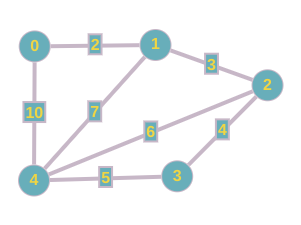
\includegraphics[width=0.4\textwidth]{Images/graph1.png}
    \caption{Grafo 1.}\label{fig:grafo1}
\end{figure}

\begin{table}[H]
    \centering
    \begin{tabular}{cccccccc}
        \toprule
        \textbf{Iteration} & \textbf{S} & \textbf{w} & \textbf{D[w]} &
        \textbf{D[1]} & \textbf{D[2]} & \textbf{D[3]} & \textbf{D[4]} \\
        \midrule
        Initial & {0} & - & - & 2 & +\infty & +\infty & 10 \\
        1 & {0,1} & 1 & 2 & 2 & 5 & +\infty & 9 \\
        2 & {0,1,2} & 2 & 5 & 2 & 5 & 9 & 9 \\
        3 & {0,1,2,3} & 3 & 9 & 2 & 5 & 9 & 9 \\
        4 & All & 4 & 9 & 2 & 5 & 9 & 9 \\
        \bottomrule
    \end{tabular}
    \caption{Esecuzione del algoritmo di Dijkstra per il nodo 0 sul grafo 1}\label{tab:Tgrafo1}
\end{table}

\clearpage
\subsection*{Esempio 2}
\begin{itemize}
    \item \textbf{Input}: 7 acquedotti, 8 tubazioni, partenza da S=0, arrivo a T=6.
    
    \item \textbf{Output}: La minima perdita da 0 a 6 è $19ml/s$.
\end{itemize}

\begin{figure}[h!]
    \centering
    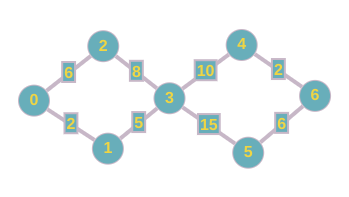
\includegraphics[width=0.4\textwidth]{Images/graph2.png}
    \caption{Grafo 2.}\label{fig:grafo2}
\end{figure}

\begin{table}[H]
    \centering
    \begin{tabular}{cccccccccc}
        \toprule
        \textbf{Iteration} & \textbf{S} & \textbf{w} & \textbf{D[w]} &
        \textbf{D[1]} & \textbf{D[2]} & \textbf{D[3]} & \textbf{D[4]} &
        \textbf{D[5]} & \textbf{D[6]} \\
        \midrule
        Initial & 0 & - & - & 2 & 6 & +\infty & +\infty & +\infty & +\infty \\
        1 & {0,1} & 1 & 2 & 2 & 6 & 7 & +\infty & +\infty & +\infty \\
        2 & {0,1,2} & 2 & 6 & 2 & 6 & 7 & +\infty & +\infty & +\infty \\
        3 & {0,1,2,3} & 3 & 7 & 2 & 6 & 7 & 17 & 22 & +\infty \\
        4 & {0,1,2,3,4} & 4 & 17 & 2 & 6 & 7 & 17 & 22 & 19 \\
        5 & All & 6 & 19 & 2 & 6 & 7 & 17 & 22 & 19 \\
        \bottomrule
    \end{tabular}
    \caption{Esecuzione del algoritmo di Dijkstra per il nodo 0 sul grafo 2}
\end{table}

\clearpage
\subsection*{Esempio 3}
\begin{itemize}
    \item \textbf{Input}: 9 acquedotti, 14 tubazioni, partenza da S=0, arrivo a T=8.
    \item \textbf{Output}: La minima perdita da 0 a 8 è $14ml/s$.
\end{itemize}

\begin{figure}[h!]
    \centering
    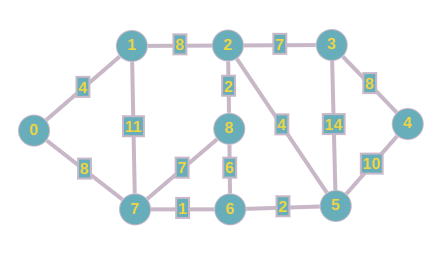
\includegraphics[width=0.4\textwidth]{Images/graph3.png}
    \caption{Grafo 3.}\label{fig:grafo3}
\end{figure}

\begin{table}[H]
    \centering
    \resizebox{\textwidth}{!}{ % Ridimensiona la tabella alla larghezza del testo
    \begin{tabular}{cccccccccccc}
        \toprule
        \textbf{Iteration} & \textbf{S} & \textbf{w} & \textbf{D[w]} & 
        \textbf{D[1]} & \textbf{D[2]} & \textbf{D[3]} & \textbf{D[4]} & 
        \textbf{D[5]} & \textbf{D[6]} & \textbf{D[7]} & \textbf{D[8]} \\
        \midrule
        Initial & 0 & - & - & 4 & +\infty & +\infty & +\infty & +\infty & +\infty & 8 & +\infty \\
        1 & {0,1} & 1 & 4 & 4 & 12 & +\infty & +\infty & +\infty & +\infty & 8 & +\infty \\
        2 & {0,1,7} & 7 & 8 & 4 & 12 & +\infty & +\infty & +\infty & 9 & 8 & 15 \\
        3 & {0,1,7,6} & 6 & 9 & 4 & 12 & +\infty & +\infty & 11 & 9 & 8 & 15 \\
        4 & {0,1,7,6,5} & 5 & 11 & 4 & 12 & 25 & 21& 11 & 9 & 8 & 15 \\
        5 & {0,1,7,6,5,2} & 2 & 12 & 4 & 12 & 19 & 21& 11 & 9 & 8 & 14 \\
        6 & {0,1,7,6,5,2,8} & 8 & 14 & 4 & 12 & 19 & 21& 11 & 9 & 8 & 14 \\
        7 & {0,1,7,6,5,2,8,3} & 3 & 19 & 4 & 12 & 19 & 21& 11 & 9 & 8 & 14 \\
        8 & All & 4 & 21 & 4 & 12 & 19 & 21& 11 & 9 & 8 & 14 \\
    \end{tabular}
    }
    \caption{Esecuzione dell'algoritmo di Dijkstra per il nodo 0 sul grafo 3.}
\end{table}

\clearpage

\section{Complessità di tempo e spazio}
La complessità temporale dell'algoritmo di Dijkstra dipende dall'implementazione della
coda a priorità, che in questo caso è fatta tramite \textbf{Heap binario}, e dal numero 
di archi e di vertici del grafo.\\

\begin{enumerate}
    \item \textbf{Operazioni sulla coda di priorità}: 
    \begin{itemize}
        \item textbf{Inserimento}: l'inserimento di nuovi elementi nell'heap binario ha
        un costo di $\mathcal{O}(\log{V})$ necessario per mantenere l'ordinamento.
        \item \textbf{Estrazione del minimo}: l'estrazione del nodo con la distanza minima 
        ha anch'essa complessità $\mathcal{O}(\log{V})$, poichè a struttura deve essere aggiornata.
    \end{itemize}

    \item \textbf{Esplorazione del grafo}:
    \begin{itemize}
        \item Dijkstra visita ogni nodo una volta, quindi esegue al massimo $V$ operazini di pop
        dalla coda. Inoltre esamina ogni arco una volta per aggiornare le distanze.
        Ogni arco comporta un'operazione di push o un aggiornamento di un nodo nella coda. 
        Poiché l'inserimento e l'aggiornamento nella coda di priorità hanno complessità 
        $\mathcal{O}(\log{V})$, e ci sono $E$ archi, in totale eseguiamo $E$ operazioni 
        di push.
    \end{itemize}
\end{enumerate}

Riassumendo, si ha in totale na complessità temporale di $\mathcal{O}(E + V \log{V})$.

In termini di complessità spaziale, il grafo è rappresentato con una lista 
di adiacenza che occupa $O(V+E)$. La coda con priorità memorizza fino a $V$ nodi, 
il che porta la complessità spaziale complessiva a $O(V+E)$. 
Questa complessità è ottimale per il problema, dato il limite 
sugli acquedotti ($n \leq 200$) e sui tubi ($m \leq 5000$).

\section{Strutture dati utilizzate}
Per rappresentare il grafo, ho utilizzato due possibili rappresentazioni:
\begin{itemize}
    \item \textbf{Lista di adiacenza}: Questa struttura è stata utilizzata per ridurre lo 
    spazio necessario per grafi sparsi. Permette di memorizzare efficientemente i vicini di 
    ogni nodo e le loro perdite associate.
    \item \textbf{Matrice di adiacenza}: Utilizzata per rappresentare grafi più densi, anche 
    se meno efficiente in termini di spazio.
\end{itemize}

Per la gestione della selezione del nodo successivo con la minima distanza, è stata 
utilizzata una \textbf{coda con priorità} implementata come min-heap, che permette 
l'accesso al nodo con il peso minore in tempo $O(\log V)$. Questo garantisce che 
l'algoritmo funzioni in modo efficiente anche con un numero elevato di nodi.
\end{document}
